\begin{abstract}
Scaling large models requires optimization strategies that ensure rapid convergence grounded in stability. Maximal Update Parametrization ($\boldsymbol{\mu}$P) provides a theoretical safeguard for width-invariant $\Theta(1)$ activation control, whereas emerging optimizers like Muon are only ``half-aligned'' with these constraints: they control updates but allow weights to drift. To address this limitation, we introduce the \textbf{Spectral Sphere Optimizer (SSO)}, which enforces strict module-wise spectral constraints on both weights and their updates. By deriving the steepest descent direction on the spectral sphere, SSO realizes a fully $\boldsymbol{\mu}$P-aligned optimization process. To enable large‑scale training, we implement SSO as an efficient parallel algorithm within Megatron. Through extensive pretraining on diverse architectures, including Dense 1.7B, MoE 8B-A1B, and 200-layer DeepNet models, SSO consistently outperforms AdamW and Muon. Furthermore, we observe significant practical stability benefits, including improved MoE router load balancing, suppressed outliers, and strictly bounded activations.

\end{abstract}
\begin{figure}[ht]
    \centering
    \begin{subfigure}{0.48\linewidth}
        \centering
        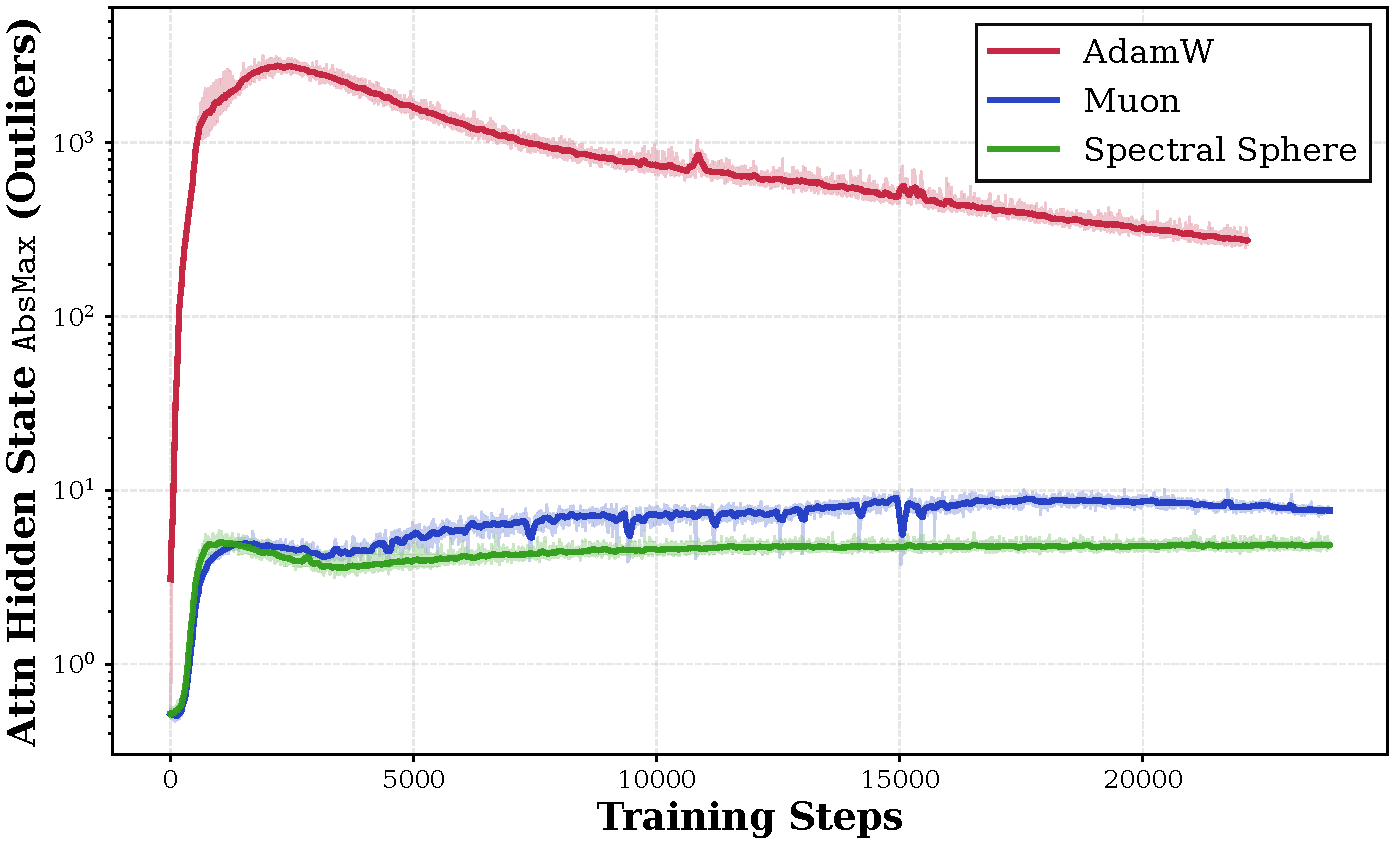
\includegraphics[width=\linewidth]{figures/exp/hsmax_attn.pdf}
        \caption{\texttt{AbsMax} (outliers) of Attention Activations}
    \end{subfigure}
    \hfill
    \begin{subfigure}{0.48\linewidth}
        \centering
        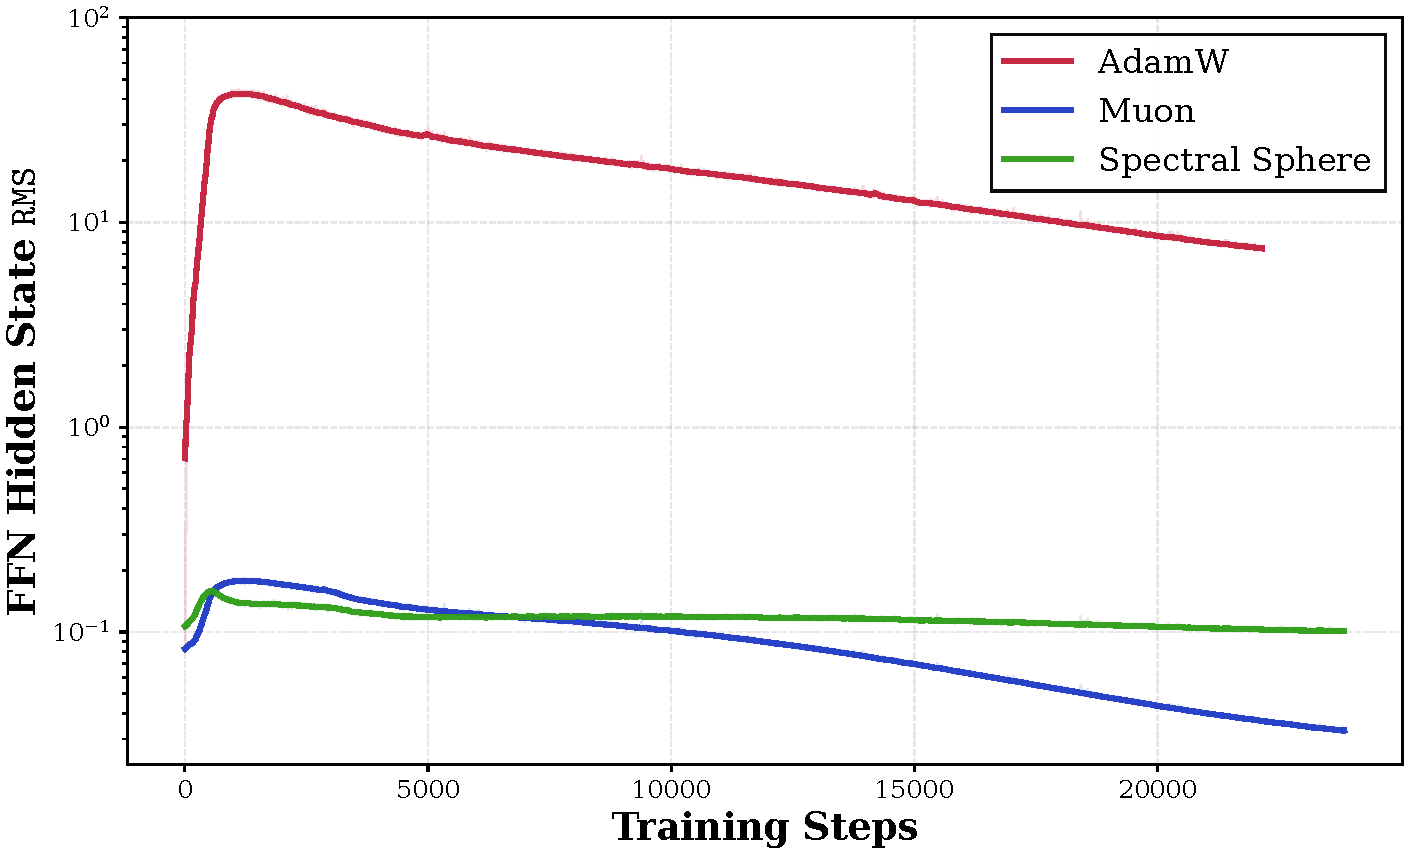
\includegraphics[width=\linewidth]{figures/exp/hsrms_mlp.pdf}
        \caption{\texttt{RMS} of FFN Activations}
    \end{subfigure}
    \caption{\textbf{Training dynamics of Dense-1.7B activations (log-scaled cross-layer averages).}
    Our \textcolor{SpectralSphereColor}{Spectral Sphere} maintains constant activation magnitudes throughout training because its $\boldsymbol{\mu}$P-metrized constraints on the spectral manifold ensure that the activation \texttt{RMS} remains at $\Theta(1)$ scale. \textcolor{MuonColor}{Muon} activations show a mild drift due to learning rate decay and weight decay. By contrast, \textcolor{AdamWColor}{AdamW} proves the most unstable, generating significantly larger activations, with attention \texttt{AbsMax} and FFN \texttt{RMS} reaching $\sim\!100\times$ magnitude compared to those spectral optimizers.}
    \label{fig:hidden_state_tracker}
\end{figure}
